\documentclass[a4paper]{article}
\usepackage[english]{babel}
\usepackage{graphicx}
\usepackage{multicol}
\usepackage{amsmath}
\usepackage{scrextend}
\usepackage[colorinlistoftodos]{todonotes}
\usepackage{blindtext}
\newcommand*{\Scale}[2][4]{\scalebox{#1}{$#2$}}%
\newcommand*{\Resize}[2]{\resizebox{#1}{!}{$#2$}}%
\usepackage{enumitem}
\usepackage{listingsutf8}
\usepackage{listings}
\usepackage{soul}
\usepackage{float}
\usepackage{epstopdf}
\usepackage{subfig}
\usepackage{amssymb}
\setlist{leftmargin=5.5mm}
\usepackage[all]{xy}
\usepackage{pdflscape}
\usepackage{longtable} 
\usepackage{cite}
\usepackage[hyphens]{url}
\usepackage[hidelinks]{hyperref}
\hypersetup{breaklinks=true}
\urlstyle{same}
\newcommand{\HRule}{\rule{\linewidth}{0.5mm}}
\usepackage{pythonhighlight}
\usepackage{xcolor}
\lstset{basicstyle=\ttfamily,
  showstringspaces=false,
  commentstyle=\color{red},
  keywordstyle=\color{blue}}
\usepackage{setspace}
\setlength{\intextsep}{3mm}
\usepackage{xcolor}
\definecolor{seagreen}{rgb}{0.18, 0.55, 0.34}
\definecolor{whitesmoke}{rgb}{0.96, 0.96, 0.96}
\definecolor{verde}{rgb}{0.25,0.5,0.35}
\definecolor{jpurple}{rgb}{0.5,0,0.35}
\definecolor{darkgreen}{rgb}{0.0, 0.2, 0.13}
\usepackage[a4paper,top=3cm,bottom=2cm,left=3cm,right=3cm,marginparwidth=1.75cm]{geometry}
\definecolor{ipython_frame}{RGB}{207, 207, 207}
\definecolor{ipython_bg}{RGB}{247, 247, 247}
\definecolor{ipython_red}{RGB}{186, 33, 33}
\definecolor{ipython_green}{RGB}{0, 128, 0}
\definecolor{ipython_cyan}{RGB}{64, 128, 128}
\definecolor{ipython_purple}{RGB}{170, 34, 255}
\lstdefinelanguage{iPython}{
    morekeywords={access,and,break,class,continue,def,del,elif,else,except,exec,finally,for,from,global,if,import,in,is,lambda,not,or,pass,print,raise,return,try,while},
    morekeywords=[2]{abs,all,any,basestring,bin,bool,bytearray,callable,chr,classmethod,cmp,compile,complex,delattr,dict,dir,divmod,enumerate,eval,execfile,file,filter,float,format,frozenset,getattr,globals,hasattr,hash,help,hex,id,input,int,isinstance,issubclass,iter,len,list,locals,long,map,max,memoryview,min,next,object,oct,open,ord,pow,property,range,raw_input,reduce,reload,repr,reversed,round,set,setattr,slice,sorted,staticmethod,str,sum,super,tuple,type,unichr,unicode,vars,xrange,zip,apply,buffer,coerce,intern},
    sensitive=true,
    morecomment=[l]\#,
    morestring=[b]',
    morestring=[b]",
    morestring=[s]{'''}{'''},
    morestring=[s]{"""}{"""},
    morestring=[s]{r'}{'},
    morestring=[s]{r"}{"},
    morestring=[s]{r'''}{'''},
    morestring=[s]{r"""}{"""},
    morestring=[s]{u'}{'},
    morestring=[s]{u"}{"},
    morestring=[s]{u'''}{'''},
    morestring=[s]{u"""}{"""}
    literate=
    {á}{{\'a}}1 {é}{{\'e}}1 {í}{{\'i}}1 {ó}{{\'o}}1 {ú}{{\'u}}1
    {Á}{{\'A}}1 {É}{{\'E}}1 {Í}{{\'I}}1 {Ó}{{\'O}}1 {Ú}{{\'U}}1
    {à}{{\`a}}1 {è}{{\`e}}1 {ì}{{\`i}}1 {ò}{{\`o}}1 {ù}{{\`u}}1
    {À}{{\`A}}1 {È}{{\'E}}1 {Ì}{{\`I}}1 {Ò}{{\`O}}1 {Ù}{{\`U}}1
    {ä}{{\"a}}1 {ë}{{\"e}}1 {ï}{{\"i}}1 {ö}{{\"o}}1 {ü}{{\"u}}1
    {Ä}{{\"A}}1 {Ë}{{\"E}}1 {Ï}{{\"I}}1 {Ö}{{\"O}}1 {Ü}{{\"U}}1
    {â}{{\^a}}1 {ê}{{\^e}}1 {î}{{\^i}}1 {ô}{{\^o}}1 {û}{{\^u}}1
    {Â}{{\^A}}1 {Ê}{{\^E}}1 {Î}{{\^I}}1 {Ô}{{\^O}}1 {Û}{{\^U}}1
    {œ}{{\oe}}1 {Œ}{{\OE}}1 {æ}{{\ae}}1 {Æ}{{\AE}}1 {ß}{{\ss}}1
    {ç}{{\c c}}1 {Ç}{{\c C}}1 {ø}{{\o}}1 {å}{{\r a}}1 {Å}{{\r A}}1
    {€}{{\EUR}}1 {£}{{\pounds}}1
    {^}{{{\color{ipython_purple}\^{}}}}1
    {=}{{{\color{ipython_purple}=}}}1
    {+}{{{\color{ipython_purple}+}}}1
    *{-}{{{\color{ipython_purple}-}}}1
    {*}{{{\color{ipython_purple}$^\ast$}}}1
    {/}{{{\color{ipython_purple}/}}}1
    {+=}{{{+=}}}1
    {-=}{{{-=}}}1
    {*=}{{{$^\ast$=}}}1
    {/=}{{{/=}}}1,
    identifierstyle=\color{black}\ttfamily,
    commentstyle=\color{ipython_cyan}\ttfamily,
    stringstyle=\color{ipython_red}\ttfamily,
    keepspaces=true,
    showspaces=false,
    showstringspaces=false,
    rulecolor=\color{ipython_frame},
    frame=single,
    frameround={t}{t}{t}{t},
    framexleftmargin=6mm,
    numbers=left,
    numberstyle=\tiny\color{gray},
    backgroundcolor=\color{ipython_bg},
    basicstyle=\scriptsize,
    keywordstyle=\color{ipython_green}\ttfamily}
\setlength {\marginparwidth }{2cm}
\begin{document}
\begin{titlepage}
\center
\textsc{\LARGE Université de Pau et des Pays de l’Adour}\\[1.3cm]
\textsc{\Large Principes et architecture des réseaux }\\[0.6cm]
\textsc{\large (BUT1 RT TP G2A)}\\[0.6cm]
\HRule \\[0.4cm]
{ \huge \bfseries SAÉ - 1.02 : Réseaux informatiques}\\[0.4cm]
\HRule \\[1.5cm]
\begin{minipage}{0.4\textwidth}
\begin{flushleft} \large
\emph{Élèves :}\\[.5cm]
Alexis Déhu 
\\[.5cm]
Martin Motz\\[.5cm]
\end{flushleft}
\end{minipage}
~
\begin{minipage}{0.4\textwidth}
\begin{flushright} \large
\emph{Enseignant :} \\
Stéphane Mascaron \end{flushright}
\end{minipage}\\[3cm]
\begin{center}
\bfseries Exemplaire distribué à :\\Enseignants
\end{center} 
\vfill \mbox{}
\end{titlepage}
\vspace{1pt}
\textsc{\textbf{Préambule}} \\
Lors de ce projet nous avons volontairement pas utilisé d’applications ou de logiciels afin d'effectuer nos manipulations. Ainsi nous utilisons uniquement des commandes bash présentes nativement sur la plupart des systèmes d’exploitation utilisant ce shell.\\En conséquent, notre nombre d'étapes et de manipulations se veut plus conséquent que si nous avions utilisé des outils afin d'effectuer les mêmes actions.
\newline
\renewcommand*\contentsname{Table des matières}
\tableofcontents
\newpage
\section{Introduction au projet}
Le principe de cette Situation d'Apprentissage et d'Évaluation ("SAÉ") consiste à configurer un micro-ordinateur Raspberry Pi ("RPI") ainsi qu'une machine virtuelle ("VM") sur le réseau de l'IUT afin d'y connecter le RPI et de pouvoir y accéder depuis n'importe quelle machine du réseau local de l'IUT ("LAN") via la VM.\\Le RPI sera accessible depuis une connexion SSH et devra accéder à Internet, donc aux réseaux extérieurs ("WAN").\\\\Nous utiliserons une VM sous Ubuntu 18.04 comme système d'exploitation ("SE") pour la préparation du RPI et SE sur la VM sur laquelle le RPI sera relié.\\Un capteur de température et d'humidité sera connecté au RPI afin de récupérer ces mêmes données autour de lui.\\\\Les parties textuelles en italique ainsi que la table des matières sont interfactifs.\\\\Toutes les images utilisées sont libres de droits.\\\\Les commandes précédées d'un hashtag seront à être exécutées avec les droits administrateurs, avec l'utilisation d'un sudoer ou un compte administrateur du SE.\\\\Un script d'automatisation des étapes est aussi proposé sur mon dépot \href{}{\textit{GitHub}}.
\subsection{Attentes du SAÉ}
Le cahier des charges complet est retrouvable sur la plateforme \href{https://elearn.univ-pau.fr/course/view.php?id=18202}{\textit{Elearn}} après le renseignement de ses identifiants universitaires sur le \href{https://sso.univ-pau.fr/cas/login}{\textit{SSO}} de l'université.
\subsubsection{Matériel utilisé}
\begin{itemize}
    \item[•] Micro-ordinateur Raspberry Pi 4 (8 Go) et son alimentation
    \item[•] Carte micro SD 32 Go
    \item[•] Adaptateur micro SD vers USB A
    \item[•] Machine virtuelle Ubuntu 18.04 sous \href{http://vi4rt.univ-pau.fr/}{\textit{VI4RT}}
    \item[•] Câbles RJ45 Ethernet droits
    \item[•] Capteur DHT20 avec brins de connexion
    \item[•] Résistance 10 Kilo Ohm
\end{itemize}
\subsubsection{Solutions apportées}
Afin de répondre aux attentes du SAÉ nous allons monter une image de \href{https://www.raspberrypi.com/software/operating-systems/}{\textit{Raspberry Pi OS Lite}}, le SE propriétaire de Raspberry allégé sur notre RPI avec un nom d'utilisateur et un mot de passe personnalisés. Nous devrons aussi ouvrir le port 22 du RPI afin de pouvoir y accéder via une connexion dite SSH (Secure Shell). Sa configuration réseau sera aussi à vérifier.\\\\En suivant, sur une VM créée avec l'outil VI4RT nous allons configurer un serveur DHCP auquel nous rattacherons notre RPI afin qu'il puisse récupérer une adresse IP et d'autres informations relatives au réseau auquel il appartiendra. Nous allons aussi configurer cette VM pour permettre au RPI de communiquer avec le WAN.\\Le RPI sera accessible via une connexion SSH depuis le LAN de l'IUT et pourra être utilisé comme une machine commune avec un accès à l'extérieur.\\\\En supplément de l'accessibilité du RPI sur le réseau, un capteur y sera connecté afin de récupérer la témpérature et l'humidité ambiantes. Un programme Python lira et affichera les données reçues du capteur sur la sortie standard de la machine ayant initiée la connexion SSH sur le RPI.
\subsection{Schématisation de notre solution}
\subsubsection{Infrastructure réseau résumée}
\label{sec:rzo}
\begin{figure}[!ht]
    \centering
    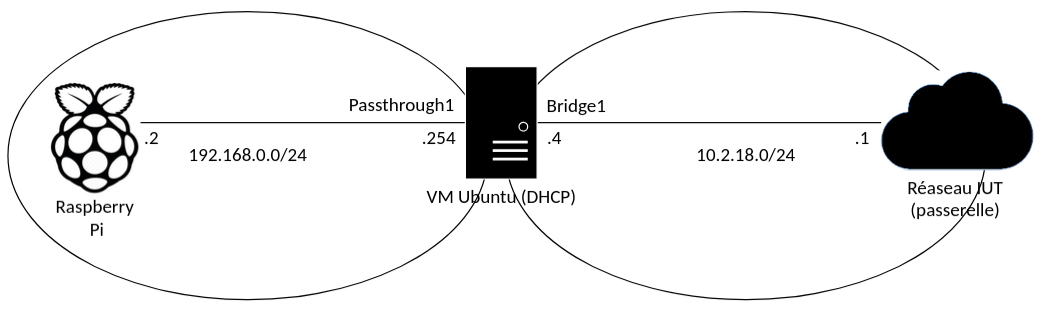
\includegraphics[scale=0.4]{rzo.png}
    \caption{Diagramme réseau simplifié de notre installation}
\label{fig:my_label}
\end{figure}
Le RPI est branché sur l'interface Passthrough1 de la VM, pas de restriction quant au masque de sous-réseau ou les adresses choisies car étant notre propre réseau local. L'adresse IP de la VM sera considérée comme celle de la passerelle par les équipements de ce LAN (192.168.0.254 sera la passerelle du réseau 192.168.0.0/24 dans notre cas).\\\\L'interface Bridge1 est reliée au réseau de l'IUT avec une adresse IP statique définie sur la plage d'adresses IP que le switch principal de l'IUT nous accorde. Ici en exemple .4, la plage d'adresse étant de 10.2.18.4 à 10.2.18.7 sur le poste TITI de la salle TP Réseaux sur lequel la configuration a été faite.\\\\Un NAT sera activé sur l'interface Bridge1 de la VM pour que le RPI puisse communiquer avec le LAN de l'IUT (10.2.18.0/24) et le WAN.
\begin{figure}[!ht]
    \centering
    \includegraphics[scale=2]{Untitled.jpg}
    \caption{Branchements sur le poste présent des salles TP Réseaux}
    \label{fig:poste}
\end{figure}
\begin{figure}[!ht]
    \centering
    
\includegraphics[scale=0.9]{baie.png}
    \caption{Branchements sur la baie de la salle}
    \label{fig:baie}
\end{figure}
\newpage
\subsubsection{Illustration connexion capteur/Raspberry Pi}
\label{sec:branchementcapteur}
Le PIN le plus à gauche du capteur vu de haut est appelé VCC, c'est-à-dire l'alimentation en +5V que fournit le pin numéro 2 dit 5V PWR du RPI.\\\\Le deuxième pin du capteur est celui des données DATA rattaché à une résistance pull-up de 10 K Ohms dans notre cas d'usage (10 K Ohms étant la valeur de résistance maximale possible, 4.7 K Ohms la minimale). Celui-ci est aussi placé sur le pin GPIO 4 afin de récupérer les données (n'importe quel pin GPIO suffit)\\\\Le quatrième et dernier pin du capteur est celui de la masse GND rattaché à la masse du RPI.
\begin{figure}[!ht]
    \centering
    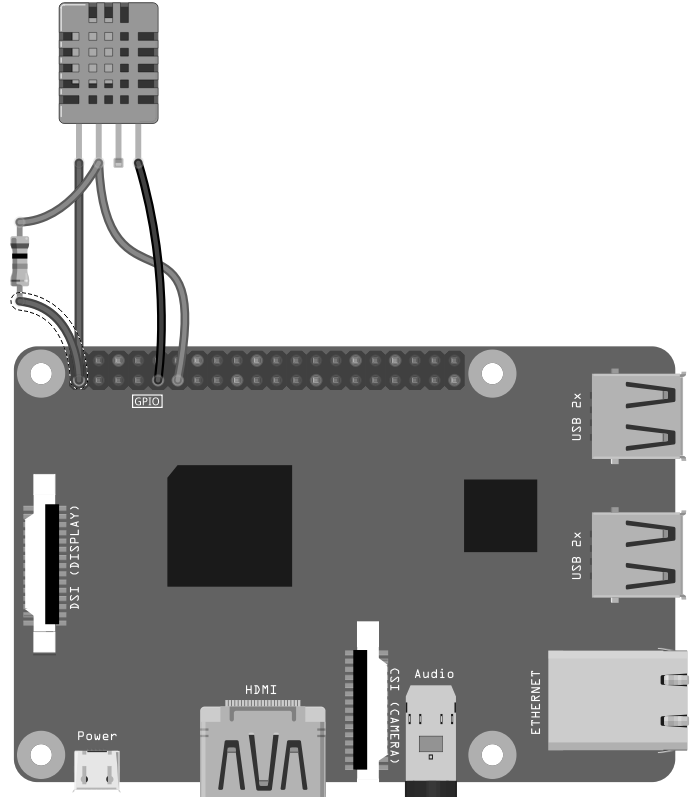
\includegraphics[scale=0.27]{grayscale_rpi1.png}
    \caption{Schéma des branchements du capteur DHT20 sur le RPI}
\end{figure}
\begin{figure}[!ht]
    \centering
    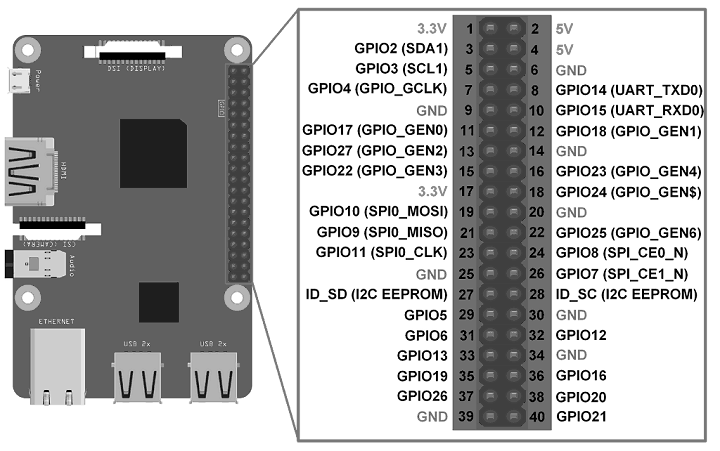
\includegraphics[scale=0.5]{gpio_pins_grayscale.png}
    \caption{Schéma des pins du RPI}
\end{figure}
\section{Préparation du Raspberry Pi}
Dans cette section nous allons configurer le RPI de manière "headless", c'est-à-dire sans périphérique d'entrée ou de sortie.\\\\Nous téléchargerons et installerons le SE pour ensuite créer un utilisateur avec un mot de passe personnalisé et enfin nous lui permettrons d'être accessible via ssh en suivant sa configuration réseau.
\subsection{Mise en place du SE}
Nous allons "flasher", installer le SE une fois téléchargé pour ensuite configurer un utilisateur avec un mot de passe chiffré.
\subsubsection{Récupération de l'image du SE}
Nous allons récupérer la dernière image en date du système d'exploitation (SE) allégé propriétaire de Raspberry pour ses Raspberry Pi: \href{https://www.raspberrypi.com/software/operating-systems/}{\textit{Raspberry Pi OS Lite}}. Nous utiliserons sa version Lite ne contenant pas d'environnement de bureau, elle utilisera moins d'espace de stockage et de ressources matérielles (ne contenant pas les paquets pour et n'exécutant pas d'interface graphique utilisateur).\\\\ Suite à cette commande, à l'emplacement du terminal, un fichier avec l'extension \verb|.iso| sera téléchargé et sera le SE avant son installation.
\definecolor{light-gray}{gray}{0.95}
\lstset{columns=fullflexible, basicstyle=\ttfamily,
    backgroundcolor=\color{light-gray},xleftmargin=0.5cm, xrightmargin=0.5cm,frame=tlbr,framesep=4pt,framerule=0pt,breaklines=true}
\begin{lstlisting}
    $ wget https://downloads.raspberrypi.org/raspios_lite_armhf/images/raspios_lite_armhf-2022-09-26/2022-09-22-raspios-bullseye-armhf-lite.img.xz
\end{lstlisting}
\label{sec:sec01}
\subsubsection{Découverte de la location du périphérique de stockage}
Afin d'installer le système d'exploitation sur la carte micro SD du RPI, ou le "flasher", nous devons connecter sa carte micro SD sur notre machine via l'adaptateur.\\Après cela nous devons trouver l'emplacement du lecteur de la carte micro SD sur notre machine.
\begin{lstlisting}
    # lshw -C disk
\end{lstlisting}
\noindent Voici un exemple de sortie de cette commande, on reconnait la micro SD de 32 Go sur /dev/sda).
\begin{lstlisting}[language=bash]
  *-disk
       description: SCSI Disk
       product: SD/MMC/MS PRO
       vendor: Generic-
       physical id: 0.0.0
       bus info: scsi@1:0.0.0
       logical name: /dev/sda
       version: 1.00
       serial: 2012062914345300
       size: 29GiB (31GB)
       capabilities: removable
       configuration: ansiversion=4 logicalsectorsize=512 sectorsize=512
     *-medium
          physical id: 0
          logical name: /dev/sda
          size: 29GiB (31GB)
  *-namespace:0
       description: NVMe disk
       physical id: 1
       bus info: nvme@0:1
       logical name: /dev/nvme0n1
       size: 238GiB (256GB)
       capabilities: gpt-1.00 partitioned partitioned:gpt
       configuration: guid=a60f757c-dcfd-4648-b132-fcfdc5ba2205 
       logicalsectorsize=512 
       sectorsize=512 wwid=eui.01000000000000008ce38e0400a37168
\end{lstlisting}
\subsubsection{Installation de l'image du SE sur la carte micro SD}
Nous avons l'image du SE à "flasher" sur la carte micro SD ainsi que l'emplacement du ce périphérique de stockage. Nous devons maintenant écrire le contenu du fichier sur la carte micro SD.\\\noindent Le premier argument de la commande est l'emplacement du fichier lu, dans cette demonstration elle se situe à l'emplacement où le terminal a été lancé.\\\\La carte micro SD a comme emplacement \verb|/dev/sda| vu \hyperref[sec:sec01]{\textit{2.1.2}}.
\definecolor{light-gray}{gray}{0.95}
\begin{lstlisting}
    # xzcat 2022-09-06-raspios-bullseye-armhf-lite.img.xz | dd bs=4M of=/dev/sda
\end{lstlisting}
\subsection{Configuration du SE avant son déploiement}
Dans cette section nous affecterons un utilisateur avec son mot de passe chiffré sur le SE du RPI. Nous activerons aussi le service SSH afin de pouvoir se connecter au RPI avec cet utilisateur par la suite.
\subsubsection{Création d'un utilisateur et d'un mot de passe}
\label{sec:sec03}
Afin de créer un utilisateur et un mot de passe personnalisés sur notre RPI, nous devons modifier un fichier de configuration du système d'exploitation du RPI que nous venons d'installer.\\\\Pour cela nous devons d'abord débrancher et rebrancher l'adaptateur sur la machine afin que le carte micro SD soit reconnue comme un dispositif de stockage utilisable par le SE que nous utilisons.\\Dans notre cas la carte micro SD est reconnue avec comme chemin d'accès \verb|/run/media/alexis/|, "alexis" étant le nom d'utilisateur de ma session. Elle peut être observée dans l'explorateur de fichier de votre SE.\\Nous devons ensuite modifier le fichier se trouvant dans /boot/userconf sur la carte micro SD, le chemin absolu de ce fichier dans mon cas est donc \verb|/run/media/alexis/boot/userconf|.\\\\Pour éviter de fournir le mot de passe en clair dans le fichier de configuration nous allons utiliser la commande \verb|openssl| pour générer un mot de passe chiffré étant \verb|"tprzo.40"| et l'attribuer à l'utilisateur \verb|"alexispi"| tout cela dans le fichier \verb|userconf|.
\definecolor{light-gray}{gray}{0.95}
\begin{lstlisting}
    # echo "alexispi:"$(echo "tprzo.40" | openssl passwd -6 -stdin) > /run/media/alexis/boot/userconf
\end{lstlisting}
\subsubsection{Configuration réseau}
La configuration réseau initiale de Raspberry Pi OS repose sur l'attente d'une réponse DHCP sur l'interface RJ45 Ethernet que l'on configurera par la suite.\\Cependant si vous souhaitez configurer le RPI sur son interface Wi-Fi IEEE lors son premier démarrage vous pouvez configurer le fichier \verb|etc/wpa_supplicant/wpa_supplicant.conf| présent sur la carte micro SD.\\\\Dans notre cas d'usage, nous laissons le RPI se connecter sur le LAN de l'IUT via son interface RJ45 Ethernet, nous utiliserons une VM faisant notamment office de serveur DHCP pour lui attribuer une adresse.\\\\Pas de manipulation à faire sur la configuration réseau du RPI dans notre cas.
\subsubsection{Activation du service SSH}
\indent Nous initierons par la suite une connexion SSH (Secure Shell) afin d'accéder au RPI via un shell d'une machine cliente. Nous devons lui indiquer d'activer le service ssh et d'ouvrir le port 22 avant son déploiement. Pour cela la création d'un fichier nommé \verb|ssh| dans le dossier \verb|/boot| de la carte micro SD suffit.\\\\L'emplacement du périphérique de stockage reste \verb|/run/media/alexis|.\\
\begin{lstlisting}
    $ touch /run/media/alexis/boot/ssh
\end{lstlisting}
\section{Déploiement du service DHCP}
Cette section présentera les configurations de base de la VM afin de déployer et expliquer le service DHCP (Dynamic Host Configuration Protocol) qui lui sera rattaché.
\subsection{Explications sur notre serveur DHCP}
Nous allons utiliser un service DHCP afin de donner différentes informations aux nouveaux équipements arrivant sur le réseau qui émettent une requête afin de les obtenir.\\\\Notre service DHCP distribuera les informations suivantes.
\begin{itemize}
    \item[•] L'adresse IP de la passerelle (192.168.0.254 dans notre cas)
    \item[•] Le masque de sous-réseau (/24 soit 255.255.255.0 ici)
    \item[•] Les adresses IP des serveurs dns
    \item[•] Une adresse IP allouée pour l'interface de l'équipement
\end{itemize}
Un service DHCP permet de ne pas avoir à renseigner manuellement toutes ces informations sur  chaque appareil voulant se connecter à notre LAN et empêchera des conflits d'adresses IP par inadvertance.
\subsection{Création de la machine virtuelle}
Nous allons nous servir de l'outil de virtualisation de l'IUT \href{http://vi4rt.univ-pau.fr}{\textit{VI4RT}} afin de créer notre VM Ubuntu.
\\\\Les paramètres à ajouter sur la page \textbf{Créer une machine} étant les suivants:
\begin{lstlisting}
    Nouvelle machine virtuelle

Nom de la machine: ubn1
Disque dur: Ubuntu 18.04 (15.00Go)
Processeur(s): 2 vcpus
Memoire vive: 4G
Cartes reseaux: 2
Carte 1 attachee a[...]: bridge1
Carte 2 attachee a[...]: pass1
\end{lstlisting}
Le \verb|Nom de la machine|, nombre de \verb|Processeur(s)| et de \verb|Mémoire vive| pouvant être modifiés, ceux indiqués sont seulement recommandés.
\subsection{Configuration réseau de la VM}
Avant de déployer le service dhcp nous devons configurer les interfaces de la VM afin de les rattacher à un ou des réseaux.
\subsubsection{Détection des interfaces réseaux}
\label{sec:secip}
\label{sec:sec02}
Nous allons commencer par lister nos interfaces ainsi que leur nom sur notre VM.\\
\begin{lstlisting}
    $ ip address
\end{lstlisting}
Un exemple de sortie de la commande, ici sur la VM.
\begin{lstlisting}    
    1: lo: <LOOPBACK,UP,LOWER_UP> mtu 65536 qdisc noqueue state UNKNOWN group default qlen 1000
    link/loopback 00:00:00:00:00:00 brd 00:00:00:00:00:00
    inet 127.0.0.1/8 scope host lo
       valid_lft forever preferred_lft forever
    inet6 ::1/128 scope host 
       valid_lft forever preferred_lft forever
2: ens3: <BROADCAST,MULTICAST,UP,LOWER_UP> mtu 1500 qdisc fq_codel state UP group default qlen 1000
    link/ether 52:54:00:95:5e:a8 brd ff:ff:ff:ff:ff:ff
    inet 10.2.18.4/24 brd 10.2.18.255 scope global ens3
       valid_lft forever preferred_lft forever
    inet6 2001:660:6701:30da:41e2:60b6:15a:5bce/64 scope global temporary dynamic 
       valid_lft 604515sec preferred_lft 85680sec
    inet6 2001:660:6701:30da:4316:b2a:a44c:28e0/64 scope global dynamic mngtmpaddr noprefixroute 
       valid_lft 2591879sec preferred_lft 604679sec
    inet6 fe80::e7dc:18bd:441b:2b9a/64 scope link noprefixroute 
       valid_lft forever preferred_lft forever
3: ens4: <BROADCAST,MULTICAST,UP,LOWER_UP> mtu 1500 qdisc fq_codel state UP group default qlen 1000
    link/ether 52:54:00:c7:c4:c3 brd ff:ff:ff:ff:ff:ff
    inet 192.168.0.254/24 brd 192.168.0.255 scope global ens4
       valid_lft forever preferred_lft forever
\end{lstlisting}
Dans notre cas l'interface Bridge1 est reconnue comme étant \verb|ens3| et Passthrough1 avec comme nom \verb|ens4|.
\subsubsection{Configuration des interfaces réseaux}
L'un des utilitaires de gestion d'interfaces réseaux les plus répandu et utilisé se nomme \verb|NetworkManager|. Celui-ci est notamment présent sur les distributions Debian et Ubuntu comme gestionnaire réseau par défaut.\\\\Nous allons modifier son fichier de configuration afin de définir les adresses IP, les masques de sous-réseau ainsi que la ou les passerelles que nous voulons attribuer aux interfaces de notre VM.\\\\Nous modifions le fichier de configuration de NetworkManager sur notre VM.
\begin{lstlisting}
    # nano /etc/network/interfaces
\end{lstlisting}
En appliquant l'architecture de la \hyperref[sec:rzo]{\textit{figure 1}} avec les noms des interfaces vus \hyperref[sec:sec02]{\textit{3.3.1}}.
\begin{lstlisting}
auto ens3
iface ens3 inet static
    address 10.2.18.4
    netmask 255.255.255.0
    gateway 10.2.18.1
    
auto ens4
iface ens4 inet static
    address 192.168.0.254
    netmask 255.255.255.0
\end{lstlisting}
\subsection{Installation du service}
Nous allons désormais déployer un service dhcp qui donnera un masque de sous-réseau, une adresse IP, celle de la passerelle ainsi que les adresses IP des serveurs DNS (Domain Name System) aux machines envoyant une requête DHCP.
\subsubsection{Mise à jour des paquets du système}
Avant d'installer un ou plusieurs paquets utilisant des fonctions systèmes il est préférable de les mettre à jour.\\\\Pour cela nous pouvons installer leur dernière version disponible.
\begin{lstlisting}
    # apt-get update -y
\end{lstlisting}
Sur notre VM Ubuntu 18.04 nous ne pouvons pas directement mettre à jour les paquets systèmes installés, la sortie étant une erreur de Glib de ce type.
\begin{lstlisting}
(appstreamcli:12346): GLib-CRITICAL **: 12:15:21.490: g_variant_new_variant: 
assertion 'value != NULL' failed

(appstreamcli:12346): GLib-ERROR **: 12:15:21.490: g_variant_new_parsed: 
11-13:invalid GVariant format string
Trace/breakpoint trap
E: Problem executing scripts APT::Update::Post-Invoke-Success 'if /usr/bin/test 
-w /var/cache/app-info -a -e /usr/bin/appstreamcli; then appstreamcli 
refresh-cache > /dev/null; fi'
E: Sub-process returned an error code
\end{lstlisting}
Nous pouvons cependant la corriger en demandant la réinstallation du paquet \verb|libappstream4| suite à quoi nous pourrons mettre à jour nos paquets normalement.
\begin{lstlisting}
    # apt-get install --reinstall libappstream4 -y && apt-get update -y
\end{lstlisting}
\subsubsection{Installation d'un paquet de service de DHCP}
Ubuntu ne propose pas nativement un service réseau pouvant répondre aux attentes d'un serveur DHCP, nous devons donc installer un paquet adéquat.\\\\Pour notre serveur dhcp nous allons installer un paquet intitulé \textbf{isc-dhcp-server}.
\begin{lstlisting}
    # apt-get install isc-dhcp-server -y
\end{lstlisting}
\subsection{Mise en place du service}
Nous allons maintenant configurer le service DHCP installé pour correspondre aux besoin de notre LAN.\\Afin d'éviter tout problème nous ferrons des sauvegardes avant chaque manipulations en montrant comment faire une restauration si des problèmes trop importants surviennent chez vous.
\subsubsection{Sauvegarde du fichier de configuration vierge}
Avant toute modification majeure d'une interface, nous allons sauvegarder son ancienne configuration vierge afin de pouvoir revenir dessus si besoin.\\\\Le fichier dont le chemin absolu est \verb|/etc/dhcp/dhcpd.conf| est initialement prévu pour être modifié, il n'applique aucune règle si non configuré. Nous allons l'utiliser pour créer une sauvegarde en la déplaçant vers un autre fichier.\\\\Création de la sauvegarde de la configuration DHCP vierge de l'interface.
\begin{lstlisting}
    # mv /etc/dhcp/dhcpd.conf{,.old}
\end{lstlisting}
Si besoin de la restaurer, nous pourrons supprimer l'ancienne configuration utilisée par le service et renommer l'ancienne (.old) afin qu'elle prenne sa place.\\\\Suite à cela nous pourrons redémarrer le service afin qu'il puisse prendre en considération les modifications de ses règles.\\\\
\textbf{/!\textbackslash SECURITE SI BESOIN DE RESTAURATION DE LA SAUVEGARDE}
\begin{lstlisting}
    # rm /etc/dhcp/dhcpd.conf; mv /etc/dhcp/dhcpd.conf.old /etc/dhcp/dhcpd.conf; systemctl restart isc-dhcp-server
\end{lstlisting}
\subsubsection{Modification de la configuration du service}
Maintenant que nous avons fait une copie de l'ancienne configuration de notre DHCP vierge, nous pouvons éditer celle actuelle sans crainte.\\\\Dans notre cas d'usage nous allons lui demander de distribuer des adresses IP entre 192.168.0.1 et 192.168.0.253 aux arrivants sur notre LAN - plage d'adresses maximale pour le masque de sous-réseau et l'adresse de passerelle 192.168.0.254 choisis, l'adresse en .254 étant déjà prise par notre VM qui sera indiquée comme passerelle.\\\\Le DHCP distribura aussi les adresses IP des serveurs DNS intérrogeables depuis le LAN de l'IUT (194.167.156.13 et 10.2.12.4) en plus du masque de sous-réseau /24 (255.255.255.0). Les autres paramètres étant pour le temps par défaut et maximum des bails dynamiques alloués.\\\\Nous devons définir ces paramètres dans le fichier \textbf{dhcpd.conf}, nous utiliserons encore \verb|nano|.
\begin{lstlisting}
    # nano /etc/dhcp/dhcpd.conf
\end{lstlisting}
Contenu du fichier \verb|/etc/dhcp/dhcpd.conf| après édition.
\begin{lstlisting}
default-lease-time 600;
max-lease-time 7200;
 
subnet 192.168.0.0 netmask 255.255.255.0 {
 range 192.168.0.1 192.168.0.253;
 option routers 192.168.0.254;
 option domain-name-servers 194.167.158.13, 10.2.12.4;
}
\end{lstlisting}
\subsubsection{Application et vérification de l'état du service}
Nous appliquons maintenant les paramètres rentrés dans le fichier de configuration sur l'interfazce sur laquelle nous voulons que le service DHCP soit activé.\\\\Dans notre cas l'interface voulue est \verb|ens4|, celle sur Passthrough1. Nous devons l'indiquer dans le fichier ayant pour chemin absolu \textbf{/etc/default/isc-dhcp-server}.
\begin{lstlisting}
    # nano /etc/default/isc-dhcp-server
\end{lstlisting}
Fichier après l'édition.
\begin{lstlisting}
    INTERFACESv4="ens4"
\end{lstlisting}
Nous regarderons aussi après l'application des paramètres que le service est bien actif et qu'il ne reporte aucune erreur.\\\\Si la sortie de la commande suivant affiche en vert un message \verb|active (running)|, alors le service a correctement redémarré et appliqué les paramètres que vous lui avez renseignés. Sinon des instructions ou message(s) d'erreur(s) vous serons indiqué(s).\\\\Pour redémarrer et voir le status du service nous utilisons \textbf{systemctl} (Q ou CTRL+C pour quitter)
\begin{lstlisting}
    # systemctl restart isc-dhcp-server; systemctl status isc-dhcp-server
\end{lstlisting}
Suite à celà, si l'on connecte le RPI sur l'interface Passthrough1 de la VM, celui-ci intégrera notre LAN suivant le masque de sous-réseau avec une adresse IP parmis la plage d'adresse que nous avons accordé au DHCP, une liste de deux serveurs DNS utilisables lui sera distribué ainsi que l'adresse IP de la VM en tant que passerelle du LAN.
\section{Configuration d'un NAT}
Afin que les équipements de notre LAN puisse communiquer avec ceux des autres réseaux nous devons configurer un routeur NAT (Network Address Translation) qui s'occupera de faire traverser les paquets IP aux bons destinataires de chaques réseaux.
\subsection{Explications sur le routage de paquets}
Dans cette section nous allons configurer notre VM pour faire circuler les requêtes et réponses IP des équipements connectés sur notre LAN sur les réseaux extérieurs. En d'autres termes nous allons faire accéder notre RPI au WAN, ses requêtes et les réponses attendues pour des réseaux extérieurs sortiront par la VM pour revenir vers lui.\\\\Seulement, si les équipements de notre LAN comme le RPI avaient uniquement besoin de communiquer avec d'autres équipements du réseau local, la redirection de paquets n'aurait pas été nécessaire, toutes les machines communiquant sur le même réseau.\\\\A noter que nous activons le NAT sur notre VM, les paquets IP de notre LAN pourront accéder au LAN de l'IUT et sur le WAN, notre VM pouvant communniquer avec l'extérieur.
\subsection{Paramètrage de la redirection de paquets}
L'activation du NAT passe par un routage des paquets IP sur notre réseau. Ce procédé appelé \verb|ip forward| en anglais permet de déterminer la direction que doivent prendre les paquets selon le réseau ou la machine recherché.\\\\Avec l'ip forward d'activé, notre RPI pourra accéder à des ressources ou des équipements extérieurs au LAN, il pourra envoyer sa requête IP à la passerelle, la VM dans notre cas, pour que celle-ci se charge de transmettre ce paquet là où elle le peut et renverra le retour au RPI.
\subsubsection{Activation de la variable de routage}
Afin d'activer le NAT, nous devons activer une variable système sur notre VM afin de faire circuler les paquets IP d'un réseau à un autre. Cette variable se nomme \verb|ip_forward| comme vu précédement, pour l'activer nous devons la passer à 1.\\\\Activation du routage des paquets IP.
\begin{lstlisting}
    # sysctl -w net.ipv4.ip_forward=1
\end{lstlisting}
\subsubsection{Application du NAT sur l'interface}
Nous devons désormais définir sur quelle interface l'ip foward devra être actif.\\\\Dans notre cas nous devons définir l'ip forward sur l'interface Bridge1 soit ens3 de notre VM afin que les requêtes de notre LAN puisse accéder au réseau local de l'IUT ainsi qu'au WAN et inversement.\\\\Définition de l'ip forward sur l'interface ens3 de notre VM.
\begin{lstlisting}
    # iptables -t nat -A POSTROUTING -o ens3 -j MASQUERADE
\end{lstlisting}
\subsection{Contrôles supplémentaires après configuration}
\label{sec:ici}
Même si notre installation touche à sa fin, afin d'éviter tout problème ou conflit nous allons effectuer quelques vérifications simples afin de s'assurer notre infrastructure fonctionne correctement.\\\\Ces vérifications sont optionnelles et sont mises à disposition selon votre besoin.
\subsubsection{Vérification des adresses IP}
Nous pouvons vérifier les adresses IP des interfaces de nos équipements afin de s'assurer de leur identifications sur les différents réseaux.\\\\Affichage des adresses IP des interfaces d'un équipement.
\begin{lstlisting}
    $ ip address
\end{lstlisting}
Un exemple de configuration vous a été proposé \hyperref[sec:secip]{\textit{3.3.1}}
\subsubsection{Vérification des routes IP}
Nous pouvons aussi vérifier la route que les paquets doivent prendre sur nos différents appareils.
\begin{lstlisting}
    $ ip route
\end{lstlisting}
Exemple de la sortie de la commande sur la VM.
\begin{lstlisting}
    default via 10.2.18.1 dev ens3 onlink 
    10.2.18.0/24 dev ens3 proto kernel scope link src 10.2.18.4 
    192.168.0.0/24 dev ens4 proto kernel scope link src 192.168.0.254 
\end{lstlisting}
\section{Connexion et manipulation du Raspberry Pi}
Maintenant notre infrastructure réseau opérationnelle, nous pouvons nous initier une connexion SSH au RPI et utiliser le capteur rattaché.
\subsection{Connexion et début de communication au Raspberry Pi}
Dans cette section nous allons initier une connexion SSH sur le RPI définit comme hôte. A savoir que nous pouvons renseigner l'adresse IP de la machine à joindre ou le nom d'hôte sur le réseau \verb|hostname|.\\\\Le mot de passe de l'utilisateur sur lequel vous tentez de vous connecter vous sera demandé une fois la connexion initiée.
\subsubsection{Recherche de l'appareil sur le réseau}
\label{sec:iprpi}
Avant de pouvoir initier une connexion au RPI, nous vérifions que nous pouvons communiquer avec lui sur notre réseau.\\\\Pour cela une requête ICMP (Internet Control Message Protocol) suffit afin d'essayer de le joindre sur le LAN.\\\\Envoie de requêtes icmp via la commande \verb|ping| sur le RPI.
\begin{lstlisting}
    $ ping raspberrypi.local
\end{lstlisting}
Exemple de sortie concluante de la commande. L'adresse IP vu correspond à celle du RPI sur le réseau.
\begin{lstlisting}
    SORTIE COMMANDE PING
\end{lstlisting}
Si le \verb|ping| n'arrive pas à joindre le RPI, vous pouvez vérifier votre configuration réseau sur votre VM et votre RPI vu \hyperref[sec:ici]{\textit{4.3}}
\subsubsection{Initialisation d'une connexion ssh}
En connaissance de l'adresse IP de notre RPI, nous pouvons initier proprement une connexion SSH sur celui-ci.\\\\La connexion se ferra avec l'utilisateur "alexispi" configuré \hyperref[sec:sec03]{\textit{2.2.1}} et l'adresse ip du RPI vu \hyperref[sec:iprpi]{\textit{5.1.1}}.\\\\Initialisation d'une connexion SSH sur le RPI.
\begin{lstlisting}
    $ ssh alexis@192.168.0.1
\end{lstlisting}
\subsection{Utilisation du capteur}
Maintenant connecté sur le RPI, nous pouvons commencer à interragir avec le capteur branché sur celui-ci. Nous afficherons et interprêterons les données reçues du capteur via un programme Python commenté.  
\subsubsection{Explications sur l'utilisation du capteur}
Le capteur DHT20 permet de récupérer la température et l'humidité présentes à ses alentours si alimenté. Afin de récupérer ces données nous devons le connecter au RPI sur des pins dont le schéma de branchement est présenté \hyperref[sec:branchementcapteur]{\textit{1.2.2}}. Cependant nous devons lire les données sortantes du capteur afin de les interprêter et les comprendre.
\subsubsection{Programme Python pour utiliser le capteur}
Les phrases commencées par des hashtags sont des commentaires afin de mieux comprendre l'utilité des lignes de ce programme Python.
\begin{lstlisting}[language=iPython]
import time, board, adafruit_dht

dht_device = adafruit_dht.DHT22(board.D4) # Charge le capteur sur le PIN GPIO 4

while True:
    try:
        temperature, humidity = dht_device.temperature, dht_device.humidity 
        # Recupere les donnees du capteur
        print("Temperature: " + str(temperature) + " C, Humidite: " + str(humidity) + "%", end="\r") 
        # Affiche ces donnees dans la console
    except RuntimeError: 
    # Il arrive que les donnees du capteur arrivent dans le RPI en etant corrompues, on ignore donc cette erreur
        time.sleep(2.0) # Pause de 2 secondes
        continue # On continue la boucle
    except Exception as error: 
    # Cette erreur est consideree comme grave, elle n'est pas censee arriver mais protection par precaution
        dht_device.exit() # Ferme proprement la liaison capteur-programme si erreur
        raise error # Laisse l'erreur interrompre le programme
    time.sleep(2.0) # Raffraichissement toutes les 2 secondes 
\end{lstlisting}
Exemple de sortie du programme.
\begin{lstlisting}
    Temperature: 24.2 C, Humidite: 57.7%
\end{lstlisting}
\end{document}